\section{Iteración VIII}
\subsection{Resumen}
Aquí desarrollamos una plataforma web para que los usuarios registrados puedan gestionar sus propias categorías de muebles y subir sus muebles para poder usarlos dentro de la aplicación.

\subsection{Desarrollo}
La plataforma cuenta también un login para acceder a la cuenta que el usuario creó desde la aplicación (ver figura x.xx). Tras iniciar sesión, se muestra un dashboard con todos los muebles que ha subido (ver figura x.xx) y visualizarlos en 3D (ver figura x.xx). Desde aquí el usuario puede agregar, crear, modificar y eliminar categorías y subcategorías (ver figura x.xx) y agregar muebles (ver figura x.xx). Para agregar un mueble se requiere lo siguiente
\begin{itemize}
	\item Nombre del mueble
	\item Precio
	\item Categoría
	\item Subcategoría
	\item Un ZIP con los recursos del modelo en 3D.
	\item Una imagen del  mueble
\end{itemize}
Del proceso anterior hay dos elementos de suma importancia:\par
\textbf{ZIP de modelo}.- En la raíz de este ZIP deben estar todos los archivos del modelo en \textbf{formato glTF}. \par
\textbf{Imagen del mueble}.- Es una imagen que identifique al mueble. Esta imagen se mostará en el menú de muebles al crear un escenario.\par

Esta funcionalidad cumple con un proceso de negocio general para la subida de muebles a la plataforma web (ver figura x.xx)

\begin{figure}[h!]
	\centering
	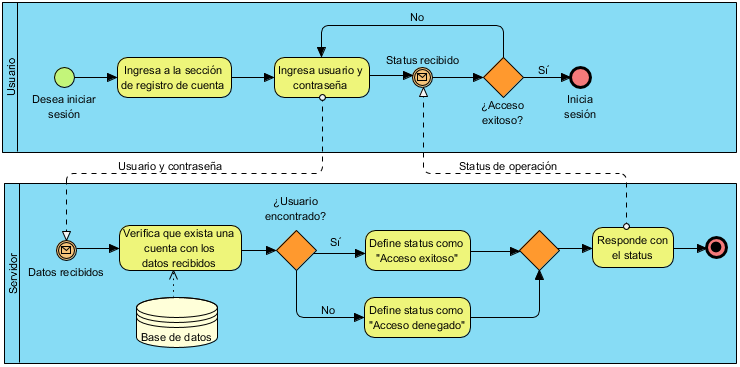
\includegraphics[width=15cm,height=9cm]{imagenes/desarrollo/diagramas/BPMN_LOGIN.png}
	\caption{Diagrama de proceso de recuperación de contraseña.}
	\label{fig:recover}
\end{figure}
\begin{figure}[h!]
	\centering
	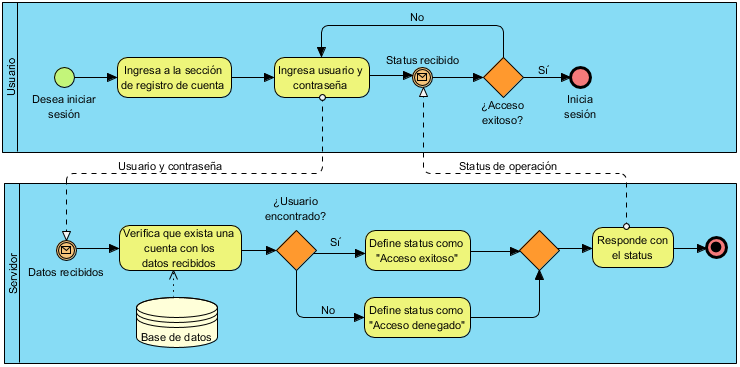
\includegraphics[width=15cm,height=9cm]{imagenes/desarrollo/diagramas/BPMN_LOGIN.png}
	\caption{Diagrama de proceso de recuperación de contraseña.}
	\label{fig:recover}
\end{figure}
\begin{figure}[h!]
	\centering
	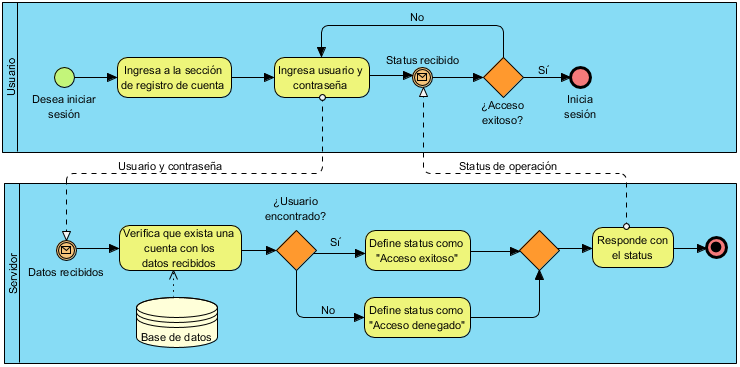
\includegraphics[width=15cm,height=9cm]{imagenes/desarrollo/diagramas/BPMN_LOGIN.png}
	\caption{Diagrama de proceso de recuperación de contraseña.}
	\label{fig:recover}
\end{figure}
\begin{figure}[h!]
	\centering
	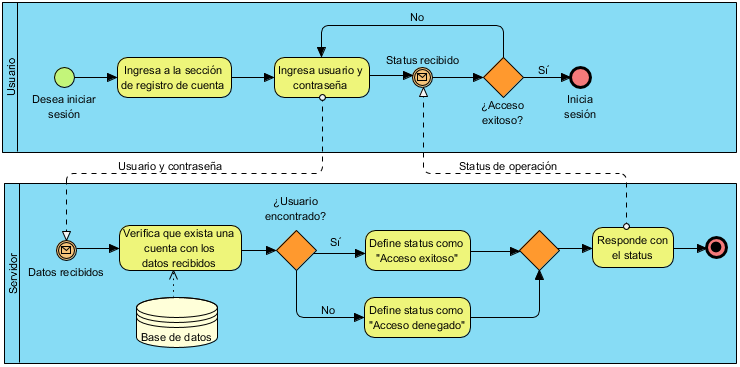
\includegraphics[width=15cm,height=9cm]{imagenes/desarrollo/diagramas/BPMN_LOGIN.png}
	\caption{Diagrama de proceso de recuperación de contraseña.}
	\label{fig:recover}
\end{figure}
\begin{figure}[h!]
	\centering
	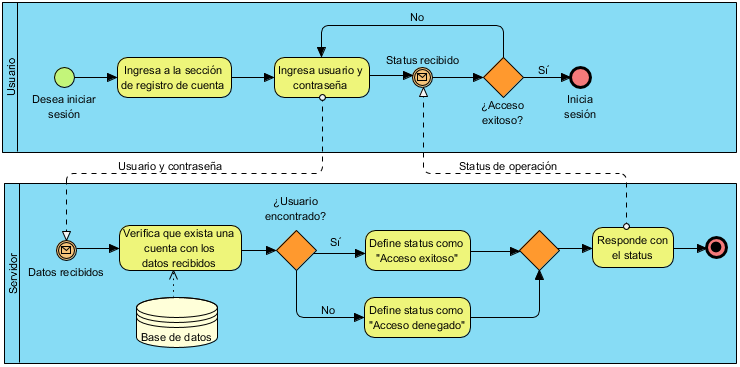
\includegraphics[width=15cm,height=9cm]{imagenes/desarrollo/diagramas/BPMN_LOGIN.png}
	\caption{Diagrama de proceso de recuperación de contraseña.}
	\label{fig:recover}
\end{figure}
\begin{figure}[h!]
	\centering
	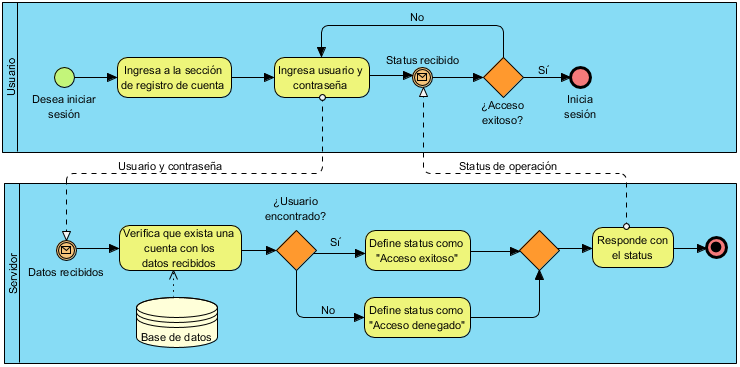
\includegraphics[width=15cm,height=9cm]{imagenes/desarrollo/diagramas/BPMN_LOGIN.png}
	\caption{Diagrama de proceso de recuperación de contraseña.}
	\label{fig:recover}
\end{figure}
\begin{figure}[h!]
	\centering
	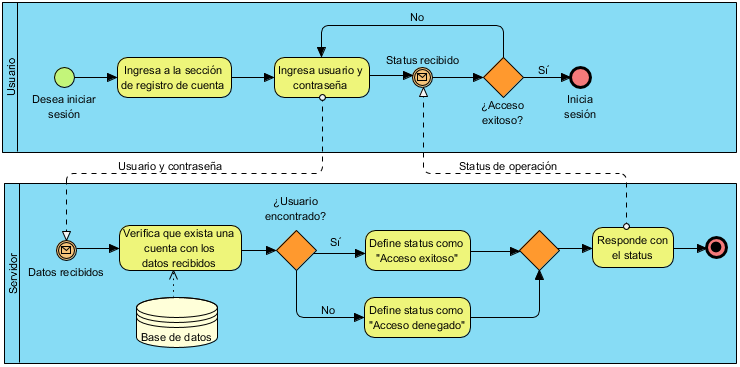
\includegraphics[width=15cm,height=9cm]{imagenes/desarrollo/diagramas/BPMN_LOGIN.png}
	\caption{Diagrama de proceso de recuperación de contraseña.}
	\label{fig:recover}
\end{figure}
